\documentclass[11pt,]{article}
\usepackage[left=1in,top=1in,right=1in,bottom=1in]{geometry}
\newcommand*{\authorfont}{\fontfamily{phv}\selectfont}
\usepackage[]{mathpazo}


  \usepackage[T1]{fontenc}
  \usepackage[utf8]{inputenc}




\usepackage{abstract}
\renewcommand{\abstractname}{}    % clear the title
\renewcommand{\absnamepos}{empty} % originally center

\renewenvironment{abstract}
 {{%
    \setlength{\leftmargin}{0mm}
    \setlength{\rightmargin}{\leftmargin}%
  }%
  \relax}
 {\endlist}

\makeatletter
\def\@maketitle{%
  \newpage
%  \null
%  \vskip 2em%
%  \begin{center}%
  \let \footnote \thanks
    {\fontsize{18}{20}\selectfont\raggedright  \setlength{\parindent}{0pt} \@title \par}%
}
%\fi
\makeatother




\setcounter{secnumdepth}{0}

\usepackage{color}
\usepackage{fancyvrb}
\newcommand{\VerbBar}{|}
\newcommand{\VERB}{\Verb[commandchars=\\\{\}]}
\DefineVerbatimEnvironment{Highlighting}{Verbatim}{commandchars=\\\{\}}
% Add ',fontsize=\small' for more characters per line
\usepackage{framed}
\definecolor{shadecolor}{RGB}{248,248,248}
\newenvironment{Shaded}{\begin{snugshade}}{\end{snugshade}}
\newcommand{\AlertTok}[1]{\textcolor[rgb]{0.94,0.16,0.16}{#1}}
\newcommand{\AnnotationTok}[1]{\textcolor[rgb]{0.56,0.35,0.01}{\textbf{\textit{#1}}}}
\newcommand{\AttributeTok}[1]{\textcolor[rgb]{0.77,0.63,0.00}{#1}}
\newcommand{\BaseNTok}[1]{\textcolor[rgb]{0.00,0.00,0.81}{#1}}
\newcommand{\BuiltInTok}[1]{#1}
\newcommand{\CharTok}[1]{\textcolor[rgb]{0.31,0.60,0.02}{#1}}
\newcommand{\CommentTok}[1]{\textcolor[rgb]{0.56,0.35,0.01}{\textit{#1}}}
\newcommand{\CommentVarTok}[1]{\textcolor[rgb]{0.56,0.35,0.01}{\textbf{\textit{#1}}}}
\newcommand{\ConstantTok}[1]{\textcolor[rgb]{0.00,0.00,0.00}{#1}}
\newcommand{\ControlFlowTok}[1]{\textcolor[rgb]{0.13,0.29,0.53}{\textbf{#1}}}
\newcommand{\DataTypeTok}[1]{\textcolor[rgb]{0.13,0.29,0.53}{#1}}
\newcommand{\DecValTok}[1]{\textcolor[rgb]{0.00,0.00,0.81}{#1}}
\newcommand{\DocumentationTok}[1]{\textcolor[rgb]{0.56,0.35,0.01}{\textbf{\textit{#1}}}}
\newcommand{\ErrorTok}[1]{\textcolor[rgb]{0.64,0.00,0.00}{\textbf{#1}}}
\newcommand{\ExtensionTok}[1]{#1}
\newcommand{\FloatTok}[1]{\textcolor[rgb]{0.00,0.00,0.81}{#1}}
\newcommand{\FunctionTok}[1]{\textcolor[rgb]{0.00,0.00,0.00}{#1}}
\newcommand{\ImportTok}[1]{#1}
\newcommand{\InformationTok}[1]{\textcolor[rgb]{0.56,0.35,0.01}{\textbf{\textit{#1}}}}
\newcommand{\KeywordTok}[1]{\textcolor[rgb]{0.13,0.29,0.53}{\textbf{#1}}}
\newcommand{\NormalTok}[1]{#1}
\newcommand{\OperatorTok}[1]{\textcolor[rgb]{0.81,0.36,0.00}{\textbf{#1}}}
\newcommand{\OtherTok}[1]{\textcolor[rgb]{0.56,0.35,0.01}{#1}}
\newcommand{\PreprocessorTok}[1]{\textcolor[rgb]{0.56,0.35,0.01}{\textit{#1}}}
\newcommand{\RegionMarkerTok}[1]{#1}
\newcommand{\SpecialCharTok}[1]{\textcolor[rgb]{0.00,0.00,0.00}{#1}}
\newcommand{\SpecialStringTok}[1]{\textcolor[rgb]{0.31,0.60,0.02}{#1}}
\newcommand{\StringTok}[1]{\textcolor[rgb]{0.31,0.60,0.02}{#1}}
\newcommand{\VariableTok}[1]{\textcolor[rgb]{0.00,0.00,0.00}{#1}}
\newcommand{\VerbatimStringTok}[1]{\textcolor[rgb]{0.31,0.60,0.02}{#1}}
\newcommand{\WarningTok}[1]{\textcolor[rgb]{0.56,0.35,0.01}{\textbf{\textit{#1}}}}
\usepackage{longtable,booktabs}

\usepackage{graphicx,grffile}
\makeatletter
\def\maxwidth{\ifdim\Gin@nat@width>\linewidth\linewidth\else\Gin@nat@width\fi}
\def\maxheight{\ifdim\Gin@nat@height>\textheight\textheight\else\Gin@nat@height\fi}
\makeatother
% Scale images if necessary, so that they will not overflow the page
% margins by default, and it is still possible to overwrite the defaults
% using explicit options in \includegraphics[width, height, ...]{}
\setkeys{Gin}{width=\maxwidth,height=\maxheight,keepaspectratio}


\title{Economic impact patterns of COVID-19 on emerging markets,
January-April/June 2020 \thanks{We gratefully acknowledge the financial support by the Dockson Chair and
the Center of International Studies at USC. Github repository:
\url{https://github.com/timodaehler/COVID19DEBT}. \textbf{Current
version:} June 09, 2020.}  }



\author{\Large Joshua Aizenman\footnote{\href{mailto:aizenman@usc.edu}{\nolinkurl{aizenman@usc.edu}}}\vspace{0.05in} \newline\normalsize\emph{Dockson Chair in Economics and IR, USC and the NBER}   \and \Large Yothin Jinjarak\footnote{\href{mailto:yothin.jinjarak@vuw.ac.nz}{\nolinkurl{yothin.jinjarak@vuw.ac.nz}}}\vspace{0.05in} \newline\normalsize\emph{School of Economics and Finance, VUW, New Zealand}   \and \Large Timo B. Dähler\footnote{\href{mailto:daehler@usc.edu}{\nolinkurl{daehler@usc.edu}}}\vspace{0.05in} \newline\normalsize\emph{SIR, USC}  }


\date{}

\usepackage{titlesec}

\titleformat*{\section}{\normalsize\bfseries}
\titleformat*{\subsection}{\normalsize\itshape}
\titleformat*{\subsubsection}{\normalsize\itshape}
\titleformat*{\paragraph}{\normalsize\itshape}
\titleformat*{\subparagraph}{\normalsize\itshape}


\usepackage{natbib}
\bibliographystyle{apsr}
\usepackage[strings]{underscore} % protect underscores in most circumstances



\newtheorem{hypothesis}{Hypothesis}
\usepackage{setspace}


% set default figure placement to htbp
\makeatletter
\def\fps@figure{htbp}
\makeatother


% move the hyperref stuff down here, after header-includes, to allow for - \usepackage{hyperref}

\makeatletter
\@ifpackageloaded{hyperref}{}{%
\ifxetex
  \PassOptionsToPackage{hyphens}{url}\usepackage[setpagesize=false, % page size defined by xetex
              unicode=false, % unicode breaks when used with xetex
              xetex]{hyperref}
\else
  \PassOptionsToPackage{hyphens}{url}\usepackage[draft,unicode=true]{hyperref}
\fi
}

\@ifpackageloaded{color}{
    \PassOptionsToPackage{usenames,dvipsnames}{color}
}{%
    \usepackage[usenames,dvipsnames]{color}
}
\makeatother
\hypersetup{breaklinks=true,
            bookmarks=true,
            pdfauthor={Joshua Aizenman\footnote{\href{mailto:aizenman@usc.edu}{\nolinkurl{aizenman@usc.edu}}} (Dockson Chair in Economics and IR, USC and the NBER) and Yothin Jinjarak\footnote{\href{mailto:yothin.jinjarak@vuw.ac.nz}{\nolinkurl{yothin.jinjarak@vuw.ac.nz}}} (School of Economics and Finance, VUW, New Zealand) and Timo B. Dähler\footnote{\href{mailto:daehler@usc.edu}{\nolinkurl{daehler@usc.edu}}} (SIR, USC)},
             pdfkeywords = {COVID-19, pandemic, emerging markets, sovereign debt},  
            pdftitle={Economic impact patterns of COVID-19 on emerging markets,
January-April/June 2020},
            colorlinks=true,
            citecolor=blue,
            urlcolor=blue,
            linkcolor=magenta,
            pdfborder={0 0 0}}
\urlstyle{same}  % don't use monospace font for urls

% Add an option for endnotes. -----


% add tightlist ----------
\providecommand{\tightlist}{%
\setlength{\itemsep}{0pt}\setlength{\parskip}{0pt}}

% add some other packages ----------

% \usepackage{multicol}
% This should regulate where figures float
% See: https://tex.stackexchange.com/questions/2275/keeping-tables-figures-close-to-where-they-are-mentioned
\usepackage[section]{placeins}


\begin{document}
	
% \pagenumbering{arabic}% resets `page` counter to 1 
%
% \maketitle

{% \usefont{T1}{pnc}{m}{n}
\setlength{\parindent}{0pt}
\thispagestyle{plain}
{\fontsize{18}{20}\selectfont\raggedright 
\maketitle  % title \par  

}

{
   \vskip 13.5pt\relax \normalsize\fontsize{11}{12} 
\textbf{\authorfont Joshua Aizenman\footnote{\href{mailto:aizenman@usc.edu}{\nolinkurl{aizenman@usc.edu}}}} \hskip 15pt \emph{\small Dockson Chair in Economics and IR, USC and the NBER}   \par \textbf{\authorfont Yothin Jinjarak\footnote{\href{mailto:yothin.jinjarak@vuw.ac.nz}{\nolinkurl{yothin.jinjarak@vuw.ac.nz}}}} \hskip 15pt \emph{\small School of Economics and Finance, VUW, New Zealand}   \par \textbf{\authorfont Timo B. Dähler\footnote{\href{mailto:daehler@usc.edu}{\nolinkurl{daehler@usc.edu}}}} \hskip 15pt \emph{\small SIR, USC}   

}

}








\begin{abstract}

    \hbox{\vrule height .2pt width 39.14pc}

    \vskip 8.5pt % \small 

\noindent With the global outbreak of COVID-19, many countries initially tried to
contain a further spread of the virus and to change the dynamics of the
pandemic with lockdowns and social distancing measures. This had two
immediate effects; On the one hand, global demand collapsed and lead to
a precipitous drop in the price for oil and other resources. On the
other hand, governments had to mitigate the economic consequences on
individuals which resulted directly from the virus or indirectly from
the government imposed lockdowns, thereby expanding government deficits
and bulking up sovereign debt. In the light of financial fragility of
emerging markets during previous global crises, this paper examines the
economic impact of the COVID-19 pandemic on government finances.
Specifically, this paper traces the cross-country associations between
COVID-19 mortality, economic fundamentals, policy interventions, and
their impact on sovereign spreads. Our results suggest\ldots{}


\vskip 8.5pt \noindent \emph{Keywords}: COVID-19, pandemic, emerging markets, sovereign debt \par

    \hbox{\vrule height .2pt width 39.14pc}



\end{abstract}


\vskip -8.5pt


 % removetitleabstract

\noindent  

\hypertarget{introduction}{%
\section{Introduction}\label{introduction}}

\hypertarget{overview}{%
\subsection{Overview}\label{overview}}

This paper takes stock of the data gathered during the first four to six
months of the year 2020. We say ``four to six'' because at the time of
writing this document (early June), the data for June is not available
yet. However, as soon as that data is available we will rerun the
analysis and see if the results remain stable. In a nutshell: we explain
the change in spread between 12/31/2019 - 04/30/2020 (and 12/31/2019 -
06/30/2020 as soon as the June data is out) through structural,
macroeconomic, and epidemiologic variables.

\hypertarget{defining-the-sample-of-countries}{%
\subsection{Defining the sample of
countries}\label{defining-the-sample-of-countries}}

In a first step, we had to choose which emerging markets we want to
investigate. Since we are interested in the effect of COVID-19 on
governments' ability to finance deficits in a sustainable way--that is,
without increasing spreads beyond reasonable levels--we are primarily
intersted in emerging markets which are ``investible''. As a starting
point, we defined a country's ``investibility'' as being a constituent
of the JPMorgan EMBI (Emerging Market Bond Index). This index gives
investors exposure to U.S. dollar-denominated government bonds issued by
emerging market countries. The index comprises more than 30 emerging
market countries in a single fund. Specifically, when we looked up the
constituent countries of the fund, it appears as if 31 countries are in
the index as of 25 April 2020 (cf.
\href{www.ishares.com/us/products/239572/ishares-jp-morgan-usd-emerging-markets-bond-etf}{https://www.ishares.com/us/products/239572/ishares-jp-morgan-usd-emerging-markets-bond-etf}
). However, some relatively large and potentially important countries
were not represented in the EMBI so that we added India and Thailand to
the sample. This results in a sample of 33 countries. We call it the
``EMBI+2'' sample. This stands in contrast to the other project we are
working on that looks at data of a 155 countries and which we call the
``extended'' sample. See the graph and table below for an overview of
the countries in the sample.

\begin{figure}
\centering
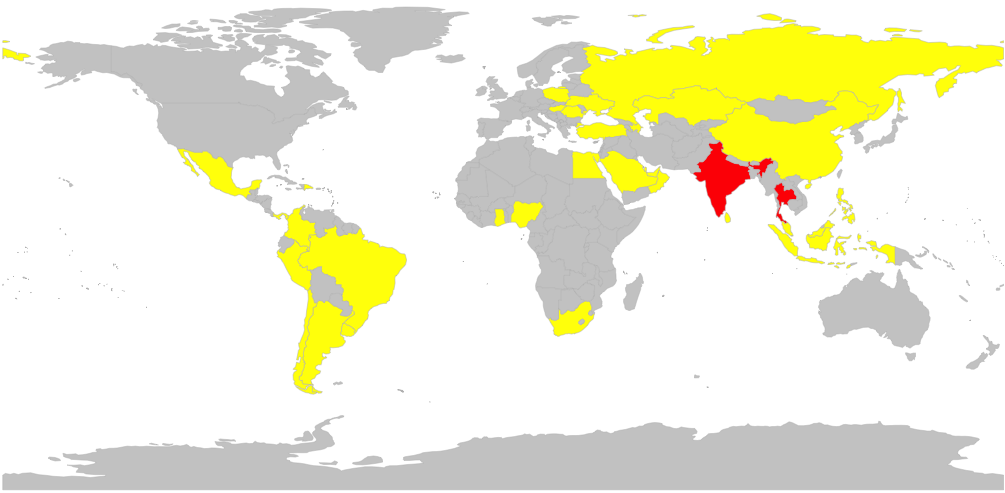
\includegraphics{reportfigures/EMBI+2.png}
\caption{EMBI+2 (Thailand \& India)}
\end{figure}

\begin{longtable}[]{@{}ll@{}}
\toprule
Country & JPM EMBI constituent (1 = yes)\tabularnewline
\midrule
\endhead
Content Cell & Content Cell\tabularnewline
Argentina & 1\tabularnewline
Azerbaijan & 1\tabularnewline
Bahrain & 1\tabularnewline
Brazil & 1\tabularnewline
Chile & 1\tabularnewline
China & 1\tabularnewline
Colombia & 1\tabularnewline
Dominican Republic & 1\tabularnewline
Egypt & 1\tabularnewline
Ghana & 1\tabularnewline
Hungary & 1\tabularnewline
India & 0\tabularnewline
Indonesia & 1\tabularnewline
Kazakhstan & 1\tabularnewline
Malaysia & 1\tabularnewline
Mexico & 1\tabularnewline
Nigeria & 1\tabularnewline
Oman & 1\tabularnewline
Panama & 1\tabularnewline
Peru & 1\tabularnewline
Philippines & 1\tabularnewline
Poland & 1\tabularnewline
Qatar & 1\tabularnewline
Romania & 1\tabularnewline
Russian Federation & 1\tabularnewline
Saudi Arabia & 1\tabularnewline
South Africa & 1\tabularnewline
Sri Lanka & 1\tabularnewline
Thailand & 0\tabularnewline
Turkey & 1\tabularnewline
Ukraine & 1\tabularnewline
United Arab Emirates & 1\tabularnewline
Uruguay & 1\tabularnewline
\bottomrule
\end{longtable}

In addition, we wanted to make sure that all the countris in the sample
are not only investable by being in the EMBI but that they also have a
certain amount of debt outstanding. To that end, we inspected the
Debt/GDP ratio of all EMBI+2 countries in the IMF's global debt database
and checked if all countries have at least a ratio of 20\%. This was
indeed the case so that we didn't drop any of the countries out of the
sample.

The rest of this document is structured as follows: The second part
outlines the data used for the analysis. The third part shows
preliminary results of correlations between the variables. The fourth
part shows regression results and graphical analyses. Part 5 concludes.

\hypertarget{data}{%
\section{2. Data}\label{data}}

In the second step, we obtained data for the outcome variable(s) and the
explanatory variables.

\hypertarget{outcome-variables}{%
\subsection{Outcome variable(s)}\label{outcome-variables}}

\begin{itemize}
\tightlist
\item
  the spread of such bonds over 1-year US treasuries
\item
  the yield of 1-year U.S. dollar-denominated bonds
\item
  the exchange rate vis-à-vis the U.S. dollar
\item
  CDS Specifically, our outcome variables are the changes of these four
  variables between the end of December 2019 and the end of April 2020
  (June 2020). While our main outcome variable of interest is the change
  in spread over U.S. bonds over 4/6 months, we also look at the other
  variables as a robustness check.
  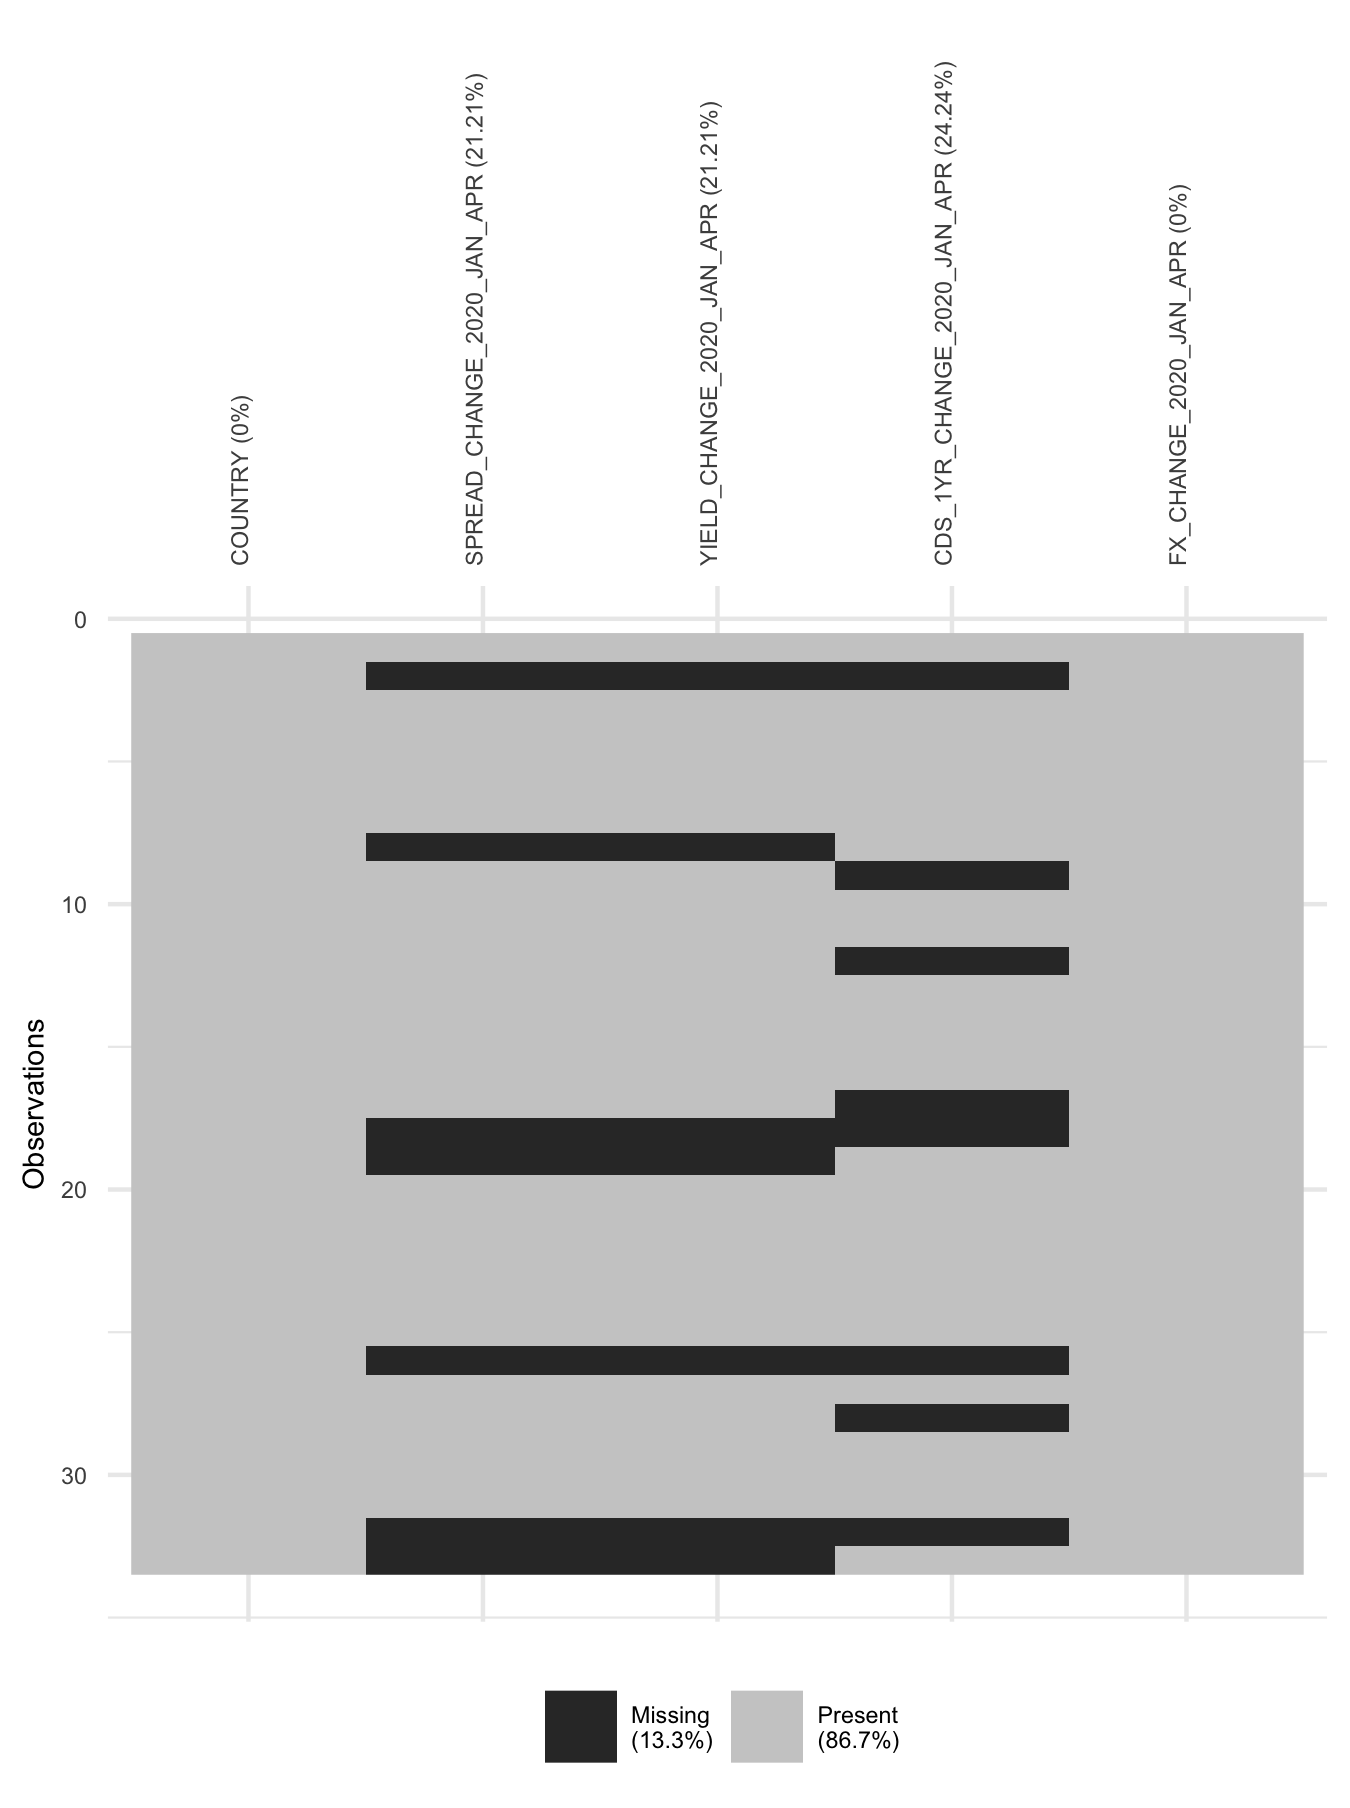
\includegraphics[width=0.5\textwidth,height=\textheight]{reportfigures/missingdata_dependentvariable.png}
\end{itemize}

\hypertarget{explanatory-variables}{%
\subsection{Explanatory variable(s)}\label{explanatory-variables}}

There are a host of explanatory variables in the dataset. Many of them
are diretly sourced from the IMF World Datamapper or from the World
Bank. However, due to the recency of the period of analysis and the lack
of officially published data, we had to hand-code a decent chunk of the
data. To do so, we looked at the IMF's country by country summary of
policy responses to COVID-19
\url{https://www.imf.org/en/Topics/imf-and-covid19/Policy-Responses-to-COVID-19}.
While the following graph does not depict all explanatory variables that
are in the dataset, it does show the most important ones which we also
expect to be the ones that show a clearn pattern in explaning the
economic fragility of emerging markets.
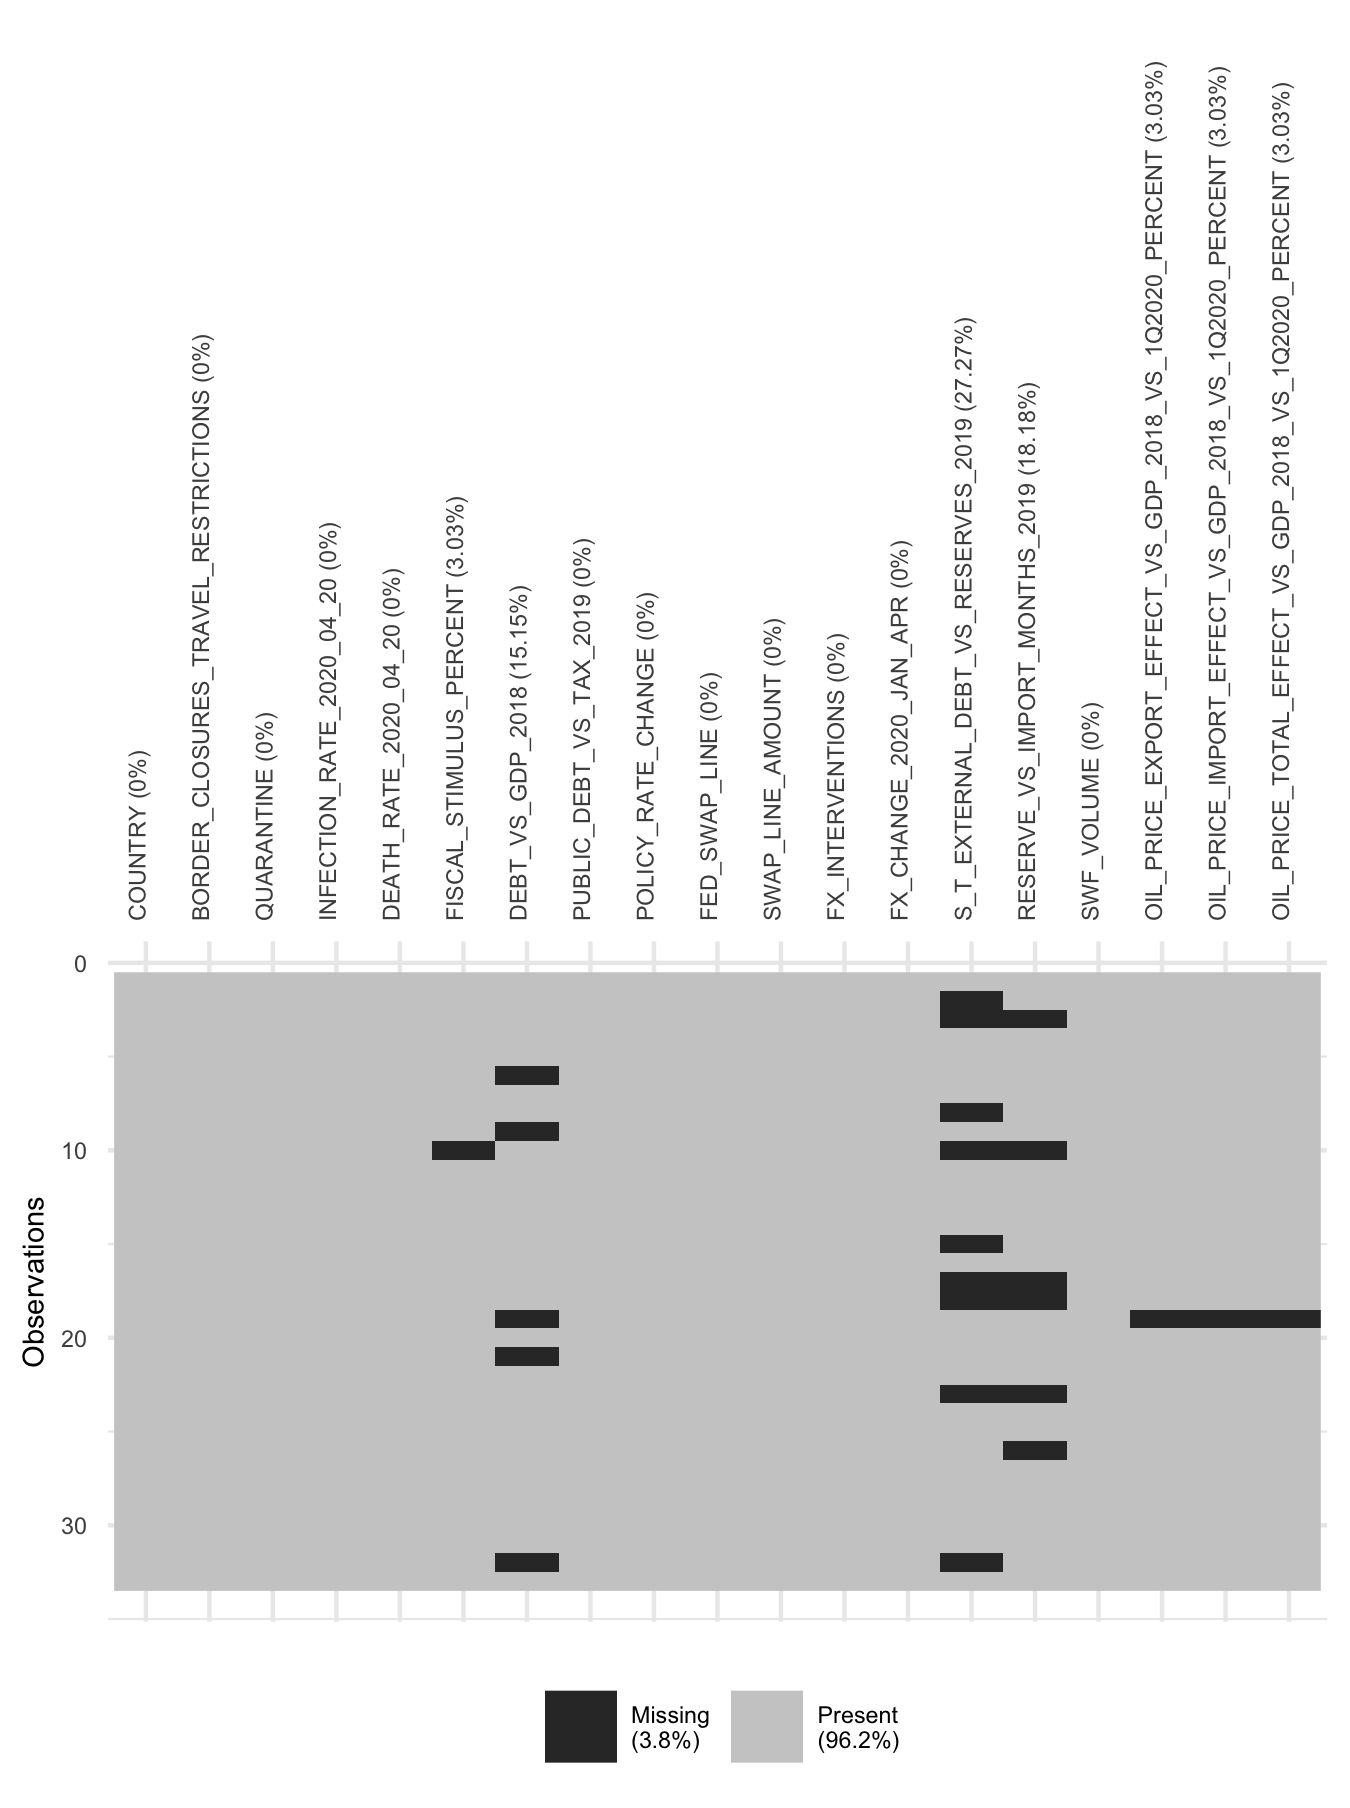
\includegraphics[width=0.5\textwidth,height=\textheight]{reportfigures/missingdata_predictors.png}

\hypertarget{data-source}{%
\subsection{Data source}\label{data-source}}

For the specific details on the variable definitions, the sources for
each variable, as well as units and further information, see the sheet
``codebook'' in the document ``data.xlsx''.

\hypertarget{preliminary-patterns-and-correlations}{%
\section{3. Preliminary patterns and
correlations}\label{preliminary-patterns-and-correlations}}

\hypertarget{econometric-results}{%
\section{4. Econometric results}\label{econometric-results}}

\hypertarget{conclusion}{%
\section{5. Conclusion}\label{conclusion}}

This is an R Markdown document. Markdown is a simple formatting syntax
for authoring HTML, PDF, and MS Word documents. For more details on
using R Markdown see \url{http://rmarkdown.rstudio.com}.

When you click the \textbf{Knit} button a document will be generated
that includes both content as well as the output of any embedded R code
chunks within the document. You can embed an R code chunk like this:

\begin{Shaded}
\begin{Highlighting}[]
\KeywordTok{summary}\NormalTok{(cars)}
\end{Highlighting}
\end{Shaded}

\begin{verbatim}
##      speed           dist       
##  Min.   : 4.0   Min.   :  2.00  
##  1st Qu.:12.0   1st Qu.: 26.00  
##  Median :15.0   Median : 36.00  
##  Mean   :15.4   Mean   : 42.98  
##  3rd Qu.:19.0   3rd Qu.: 56.00  
##  Max.   :25.0   Max.   :120.00
\end{verbatim}

\hypertarget{including-plots}{%
\section{Including Plots}\label{including-plots}}

You can also embed plots, for example:

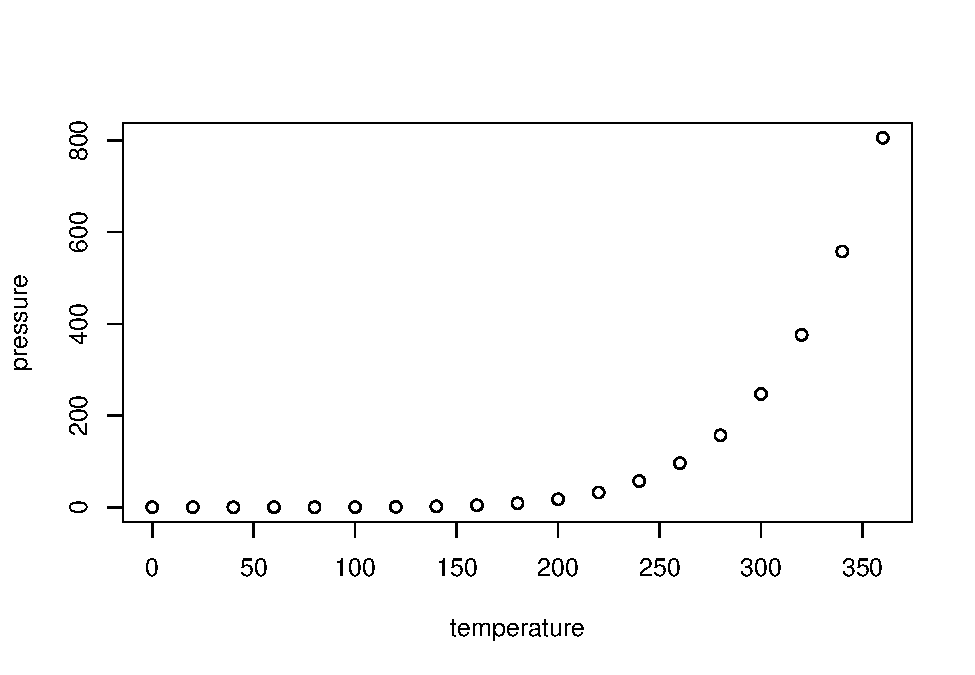
\includegraphics{Report_files/figure-latex/pressure-1.pdf}

Note that the \texttt{echo\ =\ FALSE} parameter was added to the code
chunk to prevent printing of the R code that generated the plot.

\newpage
\singlespacing 
\bibliography{/Users/timodaehler/Desktop/COVID19DEBT/Text/Bibliography.bib}
\end{document}